% Impostazioni principali
\documentclass[t, compress, mathserif]{beamer}



%         ----------------------------------------------         %
%        /                                              \        %
%--------               START PREAMBLE                   --------%
%        \                                              /        %
%         ----------------------------------------------         %

% Titolo che appare nella prima slide del documento
\newcommand{\titolo}{Analysis Of Variance}
\newcommand{\sottotitolo}{}

% Titolo che appare nella barra in basso di ogni slide, al centro
% Sono due variabili:
% * una puo' essere utilizzata per l'intero corso. Se impostata nel preambolo sovrascrive quella di seguito.
% * l'altra puo' identificare ciascun documento
\newcommand{\titolocompleto}{Statistics Course - }
\newcommand{\titoloshort}{\titolo}

% Numero di capitolo o altro nome che appare in basso di ogni slide, vicino al numero di pagina
\newcommand{\numerocapitolo}{Chapter 4}

% Include il documento che contiene il preambolo

%%%%%%%%%%%%%%%%%%%%%%%%%%%%%%%%%%%%%%%%%%%%%%%%%%%%%%%%%%%%%%%%%%%%%%%%%%%%%%
%%%%%%%%%%%%%%%%%%%%%%%%%%%% VARIABILI DA DEFINIRE %%%%%%%%%%%%%%%%%%%%%%%%%%%
%%%%%%%%%%%%%%%%%%%%%%%%%%%%%%%%%%%%%%%%%%%%%%%%%%%%%%%%%%%%%%%%%%%%%%%%%%%%%%

% Titolo che appare nella barra in basso di ogni slide, al centro
% Se impostato ha la precedenza rispetto a quello di ogni singola slide

%\renewcommand{\titolocompleto}{}

% non c'e' newcommand{\sottotitolo} perche' viene definito in ogni slide
\newcommand{\data}{}



%%%%%%%%%%%%%%%%%%%%%%%%%%%%%%%%%%%%%%%%%%%%%%%%%%%%%%%%%%%%%%%%%%%%%%%%%%%%%%
%%%%%%%%%%%%%%%%%%%%%%%%%%%%%%%%%% PACKAGES %%%%%%%%%%%%%%%%%%%%%%%%%%%%%%%%%%
%%%%%%%%%%%%%%%%%%%%%%%%%%%%%%%%%%%%%%%%%%%%%%%%%%%%%%%%%%%%%%%%%%%%%%%%%%%%%%
\usepackage[latin1]{inputenc}   
\usepackage{graphicx}
\usepackage{rotating}
\usepackage{rotfloat}
\usepackage{color}
\usepackage{colortbl}
\usepackage{../includeTex/floatflt}
\usepackage{tikz}
\usepackage{hyperref}
\usepackage{pgfpages} 
\usepackage{ifthen}
\usepackage{wasysym}
\usepackage{multirow}



%%%%%%%%%%%%%%%%%%%%%%%%%%%%%%%%%%%%%%%%%%%%%%%%%%%%%%%%%%%%%%%%%%%%%%%%%%%%%%
%%%%%%%%%%%%%%%%%%%%%%%%%%%% IMPOSTAZIONI GENERALI %%%%%%%%%%%%%%%%%%%%%%%%%%%
%%%%%%%%%%%%%%%%%%%%%%%%%%%%%%%%%%%%%%%%%%%%%%%%%%%%%%%%%%%%%%%%%%%%%%%%%%%%%%

% Beamer theme
%\usetheme{CambridgeUS}      
\usetheme{Madrid}      

% Immagini da visualizzare
\newcommand{\materiale}{minitab}

% Path delle immagini
\graphicspath{{../images/}}

% Per caricare le formule matematiche con il giusto font 
% Questo sostituisce l'opzione mathserif di documentclass (obsoleta) 
\usefonttheme[onlymath]{serif}      

     

%%%%%%%%%%%%%%%%%%%%%%%%%%%%%%%%%%%%%%%%%%%%%%%%%%%%%%%%%%%%%%%%%%%%%%%%%%%%%%
%%%%%%%%%%%%%%%%%%%%%%%%%%%%%%%%%%% COLORI %%%%%%%%%%%%%%%%%%%%%%%%%%%%%%%%%%%
%%%%%%%%%%%%%%%%%%%%%%%%%%%%%%%%%%%%%%%%%%%%%%%%%%%%%%%%%%%%%%%%%%%%%%%%%%%%%%

\definecolor{grigio}{rgb}{0.46,0.48,0.48}
\definecolor{giallo}{rgb}{1,0.84,0}
\definecolor{coolred}{rgb}{0.83,0.06,0.27}
\definecolor{arancio}{rgb}{0.97,0.46,0.09}
\definecolor{verde}{rgb}{0.25,0.78,0.25}
\definecolor{qblu}{rgb}{0.24,0.27,0.74}
\definecolor{azzurro}{rgb}{0.37,0.91,0.90}

\definecolor{grigio}{rgb}{0.46,0.48,0.48}
\definecolor{blu}{rgb}{0.25,0.28,0.78}

\definecolor{sfondoScopo}{rgb}{0.75,0.785,0.83}
\definecolor{darkred}{named}{qblu}
\definecolor{blue}{named}{qblu}

\setbeamercolor{scopo}{bg=sfondoScopo}
\setbeamercolor{section in toc}{fg=black,bg=white}
\setbeamercolor{alerted text}{fg=darkred!80!gray}
\setbeamercolor{palette primary}{fg=darkred!60!black,bg=gray!30!white}
\setbeamercolor{palette secondary}{fg=darkred!70!black,bg=gray!15!white}
\setbeamercolor{palette tertiary}{bg=darkred!80!black,fg=gray!10!white}
\setbeamercolor{palette quaternary}{fg=darkred,bg=gray!5!white}

\setbeamercolor{sidebar}{fg=darkred,bg=gray!15!white}
\setbeamercolor{palette sidebar primary}{fg=darkred!10!black}
\setbeamercolor{palette sidebar secondary}{fg=white}
\setbeamercolor{palette sidebar tertiary}{fg=darkred!50!black}
\setbeamercolor{palette sidebar quaternary}{fg=gray!10!white}

\setbeamercolor{titlelike}{parent=pallette primary,fg=darkred}
\setbeamercolor{frametitle}{bg=gray!10!white}
\setbeamercolor{frametitle right}{bg=gray!60!white}

\setbeamercolor{separation line}{}
\setbeamercolor{fine separation line}{}

%% Definizione dei colori da assegnare ai box
\setbeamercolor{postit}{fg=white,bg=qblu}
\setbeamercolor{postut}{fg=qblu,bg=gray!60!white}

%% Definizione dei colori per i diagrammi
\definecolor{bloccoIniziale}{rgb}{0.94,0.93,0.48}
\definecolor{bloccoFinale}{rgb}{0.86,0.25,0.27}
\definecolor{blocco}{rgb}{0.56,0.58,0.77}
\definecolor{bloccoSospeso}{rgb}{0.94,0.81,0.36}



%%%%%%%%%%%%%%%%%%%%%%%%%%%%%%%%%%%%%%%%%%%%%%%%%%%%%%%%%%%%%%%%%%%%%%%%%%%%%%
%%%%%%%%%%%%%%%%%%%%%%%%% STRUTTURA DELLE DIAPOSITIVE %%%%%%%%%%%%%%%%%%%%%%%%
%%%%%%%%%%%%%%%%%%%%%%%%%%%%%%%%%%%%%%%%%%%%%%%%%%%%%%%%%%%%%%%%%%%%%%%%%%%%%%

% Intestazione
\setbeamertemplate{headline}
{
  \leavevmode%
  \hbox{%
  \begin{beamercolorbox}[wd=.5\paperwidth,ht=2.25ex,dp=1ex,right]{section in head/foot}%
    \usebeamerfont{section in head/foot}\insertsectionhead\hspace*{2ex}
  \end{beamercolorbox}%
  \begin{beamercolorbox}[wd=.5\paperwidth,ht=2.25ex,dp=1ex,left]{subsection in head/foot}%
    \usebeamerfont{subsection in head/foot}\hspace*{2ex}\insertsubsectionhead
  \end{beamercolorbox}}%
  \vskip0pt%
}

% Pie' di pagina
\setbeamertemplate{footline}
{
  \hbox{%
    \begin{beamercolorbox}[wd=.20\paperwidth, ht = 2.25ex, dp = 1ex, center]{palette sidebar secondary}%
      \usebeamerfont{author in head/foot}%\insertshortauthor~~(\insertshortinstitute) 
      
\includegraphics[width=1.5cm]{QUANTIDE.jpg}
    \end{beamercolorbox}%
    \begin{beamercolorbox}[wd=.57\paperwidth, ht = 2.25ex, dp = 1ex, center]{title in head/foot}%
      \usebeamerfont{title in head/foot}{\titolocompleto \titoloshort}
    \end{beamercolorbox}%
    \begin{beamercolorbox}[wd=.13\paperwidth, ht = 2.25ex, dp = 1ex, left]{date in head/foot}%
      \hspace*{0.4em} \usebeamerfont{date in head/foot} {\numerocapitolo}
    \end{beamercolorbox}%
    \begin{beamercolorbox}[wd=.10\paperwidth, ht = 2.25ex, dp = 1ex, right]{date in head/foot}%
       \usebeamerfont{date in head/foot} \insertframenumber{} / \inserttotalframenumber \hspace*{2ex} 
    \end{beamercolorbox}%
  }%
  \vskip0pt%
}



%%%%%%%%%%%%%%%%%%%%%%%%%%%%%%%%%%%%%%%%%%%%%%%%%%%%%%%%%%%%%%%%%%%%%%%%%%%%%%
%%%%%%%%%%%%%%%%%%%%%%%%%%% STILE DELLE DIAPOSITIVE %%%%%%%%%%%%%%%%%%%%%%%%%%
%%%%%%%%%%%%%%%%%%%%%%%%%%%%%%%%%%%%%%%%%%%%%%%%%%%%%%%%%%%%%%%%%%%%%%%%%%%%%%

% Simboli di navigazione
\setbeamertemplate{navigation symbols}{}

% Modifica lo stile dell'elenco (di primo livello)
\useitemizeitemtemplate{$\star$} % Usa la stella

% Interlinea (fattore di scala; NON e' un valore assoluto)
\renewcommand{\baselinestretch}{1.2}  

% Definisci stile per vettori e matrici
\newcommand{\vect}[1]{\boldsymbol{\underline{#1}}} % Grassetto e sottolineato
\newcommand{\matr}[1]{\boldsymbol{#1}} % Grassetto

% Definire stile per valore assoluto
\providecommand{\abs}[1]{\lvert#1\rvert}
\providecommand{\norm}[1]{\lVert#1\rVert}

% Cambiare il nome delle figure e delle tabelle
\renewcommand{\figurename}{Figura}
\renewcommand{\tablename}{Tabella}

% Definizione sezioni, ecc.
\newcommand{\livelloA}{\section}
\newcommand{\livelloB}{\subsection}
\newcommand{\livelloC}{\subsubsection}

% Livello di profondita' del 'content panel' del PDF
% \hypersetup{bookmarksdepth=4} % il valore di default va bene

% Definizione prima slide
\title{\textbf{\titolo}}
\author{\sottotitolo}
\date{\data}






%         ----------------------------------------------         %
%        /                                              \        %
%--------               START DOCUMENT                   --------%
%        \                                              /        %
%         ----------------------------------------------         %

\begin{document}

% Pagina del titolo
\frame{\titlepage}

% Indice
% \begin{frame}
% 	 \tableofcontents
% \end{frame}

% Documento
% I soli contenuti del documento sono in un file esterno. Questo semplifica enormemente le cose qualora si volessero creare dei manuali (singoli documenti) a partire da diversi documenti.
\livelloA{Analysis of variance}

\begin{frame}
  \begin{small}
    \vspace*{.1cm}
    In the experimental research \textbf{the simultaneous comparison between the means of more than two groups} is frequent. They are composed of subjects that are undergone to different treatments or of data that have been collected in different conditions.\\
    \vspace*{.1cm}
    In order to highlight all the possible important differences among the means, \textbf{it is not correct to use Student's t-test to repeat the analysis as many times as the possible comparisons are} in couples among every single group.\\
    \vspace*{.1cm}
    With the Student's t-test, \textbf{only a part of the data is used} and therefore the power is lower.\\
    \vspace*{.1cm}
    In addition, the $ \alpha $ probability that has been chosen in order to accept the null hypothesis, or rather \textbf{the probability to commit a type I error} (that means to refuse the null hypothesis when it is true), \textbf{\ is valid only for every single comparison}.\\
    \vspace*{.1cm}
    \textbf{If there are many comparisons, the whole probability that at least one of them is significant because of the chance, is greater}.
  \end{small}
\end{frame}

\begin{frame}
  \vspace*{.25cm}
  If the $ H_0 $ null hypothesis is valid, the probability that none of the comparisons is, by chance, significant is:
  $$ (1-\alpha)^k $$
  where $ k $ \ is the number of the comparisons that have been done.\\
  \vspace*{.5cm}
  If, for example, we make 10 comparisons among the means of the groups drawn by chance from the same population and, for each of them $ \alpha $ \ is equal to 0.05, the probability that none of the comparisons is significant decreases from 0.95 to around \textbf{0.60}.\\
  \vspace*{.5cm}
  As consequence, the whole probability that at least one results to be significant, because of random fluctuations, moves from 0.05 to \textbf{0.40}.
\end{frame}

\begin{frame}
  \vspace*{.25cm}
  In different words, if we do $ k $ comparisons with the Student's t-test, each of them with $ \alpha $ probability, the whole $ \alpha' $ probability to commit at least one type I error (that the test refuses the null hypothesis even though it is true) becomes:
  $$ \alpha' = 1 - (1 - \alpha)^k $$\\
  \vspace*{.25cm}
  The analysis of variance, with an apparently words paradox, allows the comparison between two or more means.\\
  It allows the simultaneous comparison among them, \textbf{keeping unchanged the {\boldmath $ \alpha $} whole set probability}.\\
  \vspace*{.25cm}
  It represents, in addition, the core of the industrial statistics, as, for example, of the Capability or of the GAGE R\&R.
\end{frame}

\begin{frame}
  \vspace*{.25cm}
  The $ H_0 $ null hypothesis and the $ H_A $ alternative hypothesis have a more general formula, compared to the comparison between two means: \\
  \vspace*{.15cm}
  {\boldmath $$ H_0: \; \mu_1= \mu_2 = \dots = \mu_p $$}
  {\boldmath $$ H_A: \, \exists \, i,j \,\mid\,\mu_i\neq\mu_j\;\;\;(i,j=1,\,\dots,\,p)$$}\\
  \vspace*{.15cm}t of 
  Beyond the mathematical notation, the alternative hypothesis is that \textbf{at least one} of the means is different from the others.\\
  \textbf{The developed methodology to check the statistical significance of the diffences among the arithmetical means of a series of the groups, is called analysis of variance} and it is marked as \textbf{ANOVA}. It uses \textbf{the F(p,q) distribution where p and q are needed parameters to specify it}.
\end{frame}

\begin{frame}
  \vspace*{.25cm}
  \textbf{Example}. \\
  \vspace*{.15cm}
  We have an establishment with 3 parallel production lines (A, B, C) that produces silicon wafers.\\
  It wants to be checked that the mean resistivity of each of them is the same.\\
  \vspace*{.75cm}
  This is a scheme of hypothesis:\\
  \hspace*{2cm}$H_0:\;\mu_A=\mu_B=\mu_C=\mu_{TOT}$\\
  \vspace*{.15cm}
  \hspace*{2cm}$H_A:\;\exists\,\mu_j \ne \mu_{TOT}$
\end{frame}

\begin{frame}
  \vspace*{.25cm}
  In the analysis of variance, the root or the cause of the data variations is called \textbf{experimental factor} or \textbf{treatment}; it can have:
  \vspace*{.25cm}
  \begin{itemize}
    \item more quantitative \textbf{levels}, as long as it is possible to discretize them;
    \vspace*{.25cm}
    \item more qualitative \textbf{levels} (or \textbf{methods}).
  \end{itemize}
  \vspace*{.25cm}
  Every unit or observation inside the experimental observations' levels are \textbf{replication o repetition}.\\
  \vspace*{.25cm}
  In order to calculate the mean and the variance, every group must be made of at least two replications.
\end{frame}



\livelloA{One factor analysis of variance}

\begin{frame}
  \vspace*{.5cm}
  The easiest analysis of variance model, that can be seen as an extension of the Student's t-test with many independent samples, is called \textbf{one criteria classification (one way)}, or \textbf{one factor}.\\
  \vspace*{.75cm}
  For the statistics analysis, in this model \textbf{it is not required that the various groups have the same number {\boldmath $ (n_j) $} of observations or replications}.\\
  \vspace*{.75cm}
  The observations' presentation methodology, already encoded, implies that experimental data, that have been collected, are orderly carried according to the underlying table.
\end{frame}

\begin{frame}
  \vspace*{.75cm}
  \begin{tabular}{|c|c|c|c|c|c|}
    \cline{2-6}
    \multicolumn{1}{c}{} & \multicolumn{5}{|c|}{\textbf{TREATMENTS' MODALITY}}\\ 
    \multicolumn{1}{c}{} & \multicolumn{5}{|c|}{\hspace*{.25cm}\textbf{OR LEVELS}\hspace*{.25cm}} \\ \cline{2-6}
    \multicolumn{1}{c|}{} & $T_1$ & $T_2$ & $T_3$ & $\dots$ & $T_p$\\ \hline
    \multicolumn{1}{|c|}{\hspace*{6cm}} & $x_{11}$ & $x_{12}$ & $x_{13}$ & $\dots$ & $x_{1p}$ \\ 
    \multicolumn{1}{|c|}{\textbf{EXPERIMENTAL}} & $x_{21}$ & $x_{22}$ & $x_{23}$ & $\dots$ & $x_{2p}$ \\
    \multicolumn{1}{|c|}{\textbf{UNITIES}} & $x_{31}$ & $x_{32}$ & $x_{33}$ & $\dots$ & $x_{3p}$ \\
    \multicolumn{1}{|c|}{\textbf{OR}} &  &  &  &  & \\
    \multicolumn{1}{|c|}{\textbf{REPLICATIONS}} & $\dots$ & $\dots$ & $\dots$ & $\dots$ & $\dots$\\
    \multicolumn{1}{|c|}{} & $x_{n_{1}1}$ & $x_{n_{2}2}$ & $x_{n_{3}3}$ & $\dots$ & $x_{n_{p}p}$ \\ \hline
    \multicolumn{1}{|c|}{\textbf{Treatments' means}} & $\overline{x}_{.1}$ & $\overline{x}_{.2}$ & $\overline{x}_{.3}$ & $\dots$ & $\overline{x}_{.p}$ \\ \hline
    \multicolumn{1}{|c|}{\textbf{Overall mean}} & \multicolumn{5}{|c|}{$\overline{\overline{x}}$}\\ \hline
  \end{tabular}\\
  \vspace*{.5cm}
\end{frame}

\begin{frame}
  \vspace*{.25cm}
  The \textbf{single observation} is carried with two indexes. The first one regards the position occupied inside the group. The second one regards the treatment or the group it belongs to: $ x_{ij} $. \\
  \vspace*{.5cm}
  The \textbf{mean of every group or single treatment} is overlined, with a point instead of the first index and with the group index: $ \overline{x}_{.j} $.
  Sometimes the point as first index is omitted:  $ \overline{x}_{j} $.\\
  \vspace*{.5cm}
  The \textbf{overall mean} of all the data is written with a double line and without indexes: $ \overline{\overline{x}} $.\\
  \vspace*{.5cm}
  Starting from these three quantities, deviances (\textbf{Sum of Squares}) and variances (\textbf{Mean of Squares}), useful for the analysis, are estimated.
\end{frame}

\livelloB{Deviance, degrees of freedom and variance}

\begin{frame}
  \vspace*{.25cm}
  The \textbf{total deviance} or {\boldmath $ SS_T $} (Total Sum of Squares) is the sum, over all observations, of the squared differences of each observation from the overall mean.
  $$ SS_T=\sum_{j=1}^p \sum_{i=1}^{n_j}{(X_{ij}-\overline{\overline{X}})^2} $$
  The {\boldmath$ SS_T $} defines the total variability of the sample.\\
  \vspace*{.5cm}
  The \textbf{deviance between treatments} or {\boldmath $ SS_B $} (Between Sum of Squares) is the sum of squared residuals of every group's mean from the overall mean, multiplied the number of data of the correspondent group.
  $$ SS_B=\sum_{j=1}^p{n_{j}(\overline{X}_{.j}-\overline{\overline{X}})^2} $$
\end{frame}

\begin{frame}
  \vspace*{.25cm}
  The {\boldmath  $ SS_B $} defines the variability among groups independently of the dispersion of the single observations inside every group.\\
  \vspace*{.5cm}
  The \textbf{deviance within treatments} or {\boldmath $ SS_W $} (Within Sum of Squares), also called \textbf{error}, defines the sum of squared residuals of every value of the mean of its group.
  $$ SS_W = \sum_{j=1}^p \sum_{i=1}^{n_j}{(X_{ij}-\overline{X}_{.j})^2} $$
  The {\boldmath $ SS_W $} defines the variability within every single group independently of the position of the group around the sample's overall mean. 
\end{frame}

\begin{frame}
  \vspace*{.25cm}
  It is possible to demonstrate that:
  $$ SS_T = SS_B + SS_W $$ \\
  \vspace*{.25cm}
  This equation shows that a sample's total variance, whose sample units are divided in groups, can be partitioned in two components:
  \begin{itemize}
    \item a component \textbf{``between''}, given by the variability among the groups;
    \item a component \textbf{``within''}, given by the variability within the groups. 
  \end{itemize}
  \vspace*{.25cm}
  It is possible to make a comparison with the Pythagorean theorem.
\end{frame}

\begin{frame} 
  \vspace{-.2cm}
  Some examples:
  \vspace{-.3cm}
  \begin{figure}
    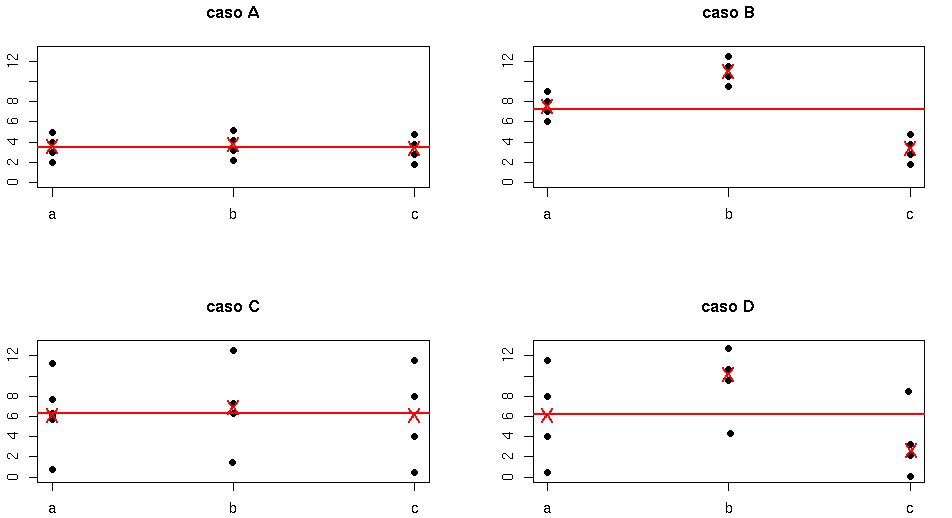
\includegraphics[height=5.5cm]{esAnova.png}
  \end{figure}
  \begin{footnotesize}
    \begin{itemize}
      \item \textbf{CASE A:} {\boldmath$ SS_W $} and {\boldmath$ SS_B $} low 
      \item \textbf{CASE B:} {\boldmath$ SS_W $} low but {\boldmath$ SS_B $} high
      \item \textbf{CASE C:} {\boldmath$ SS_W $} high but  {\boldmath$ SS_B $} low
      \item \textbf{CASE D:} {\boldmath$ SS_W $} and  {\boldmath$ SS_B $} high
    \end{itemize}
  \end{footnotesize}
\end{frame}

\begin{frame}
  \begin{small}
    \vspace*{.25cm}
    In other words, given a sample with a certain total variability, its variability components  ``within'' and ``between'' cannot change independently because their sum is bound to the total variability.\\
    \vspace*{.25cm}
    In the experimental practice, the reseacher is interested in finding a criteria that allows him to choose between the two underexposed situations can be considered true. 
    \vspace*{.25cm}
    \begin{description}
      \item[(A)]The means, calculated within the subgroups, can be considered similar among them. As consequence, the treatments to which the sample units have been undergone \textbf{did not} have any effects on the answer variable.
      \vspace*{.25cm}
      \item[(B)]The means, calculated within the subgroups, cannot be considered similar among them. As consequence, the treatments \textbf{have} had some effects on the answer variable.
    \end{description}
  \end{small}
\end{frame}

\begin{frame}
  In statistical words, the points (A) and (B) can be rewritten like follows:
  \begin{description}
    \item[(A)] All the sample units, independently of the subgroups, can be considered as they come from populations with the same mean.
      In other words, it is accepted that the factor does not have any effects on the dependent variable. In formal words, this is expressed as the null hypothesis:
      $$ H_0: \, \mu_1= \mu_2 = \mu_3 = \dots = \mu_k \mbox{.}$$ \\
    \item[(B)] \textbf{Not} all the sample units can be considered as they come from the same population or from populations with the same mean. In formal words, this is expressed as the alternative hypothesis:
      $$ H_A: \, \mbox{It exists at least one } \mu_i \mbox{ different from the others.} $$
  \end{description}
\end{frame}

\begin{frame}
  \vspace*{.25cm}
  A possible way to distinguish the case (A) and the case (B), or rather to choose if the null hypothesis $H_0$ has to be accepted or refused, consists in comparing the {\boldmath $ SS_B $} and {\boldmath $ SS_W $} between them, taking into consideration the fact that $ SS_T = SS_B + SS_W $. \\
  \vspace*{.75cm}
  If the sample means calculated within the subgroups are similar among them, then the quantity {\boldmath $SS_B$} tends to be really small.\\
  \vspace*{.25cm}
  As it is true that $ SS_T = SS_B + SS_W $, then the deviance within the subgroups {\boldmath$SS_W$} explains the great majority of the total deviance {\boldmath$SS_T$} and therefore {\boldmath$SS_W$} can be considered high compared to {\boldmath $SS_B$}.
\end{frame}

\begin{frame}
  \vspace*{.25cm}
  If, on the contrary, the sample means calculated within the subgroups are different among them, then the quantity {\boldmath$SS_B$} tends to be high.\\
  \vspace*{.25cm}
  As it is true that $ SS_T=  SS_B + SS_W $, then the variance within the subgroups {\boldmath$SS_B$} explain the great majority of the total deviance {\boldmath$SS_T$} and therefore {\boldmath$SS_B$} can be considered high compared to {\boldmath$SS_W$}.
\end{frame}

\begin{frame}
  \vspace*{.25cm}
  A possible way to distinguish between the cases (A) and (B) consists in comparing, through their ratio, the two quantities {\boldmath$SS_B$} and {\boldmath$SS_W$}.
  \vspace*{.5cm}
  \hspace*{-.5cm}
  \begin{description}
    \item[(A)] If the ratio is \textbf{small} then the means, calculated within the subgroups, can be considered \textbf{similar} among them.
    \vspace*{.5cm}
    \item[(B)] If the ratio is \textbf{high} then the means, calculated within the subgroups, can be considered \textbf{different} among them.
  \end{description}
\end{frame}

\begin{frame}
  \vspace*{.25cm}
  Unluckily, the measurements \textbf{SS} grow when the number of observations increases as they represent sum of squares' (measurements).\\
  \vspace*{.5cm}
  A possible way to avoid this problem is to consider, instead of the sum of squares (\textbf{SS}), the mean of squares (\textbf{MS}, Mean of Squares).\\
  \vspace*{.5cm}
  These measurements \textbf{MS} are obtained dividing the measurements \textbf{SS} for the correspondent degrees of freedom (\textbf{df}).
\end{frame}

\begin{frame}
  \vspace*{.5cm}
  \textbf{The degrees of freedom are estimated by the number of independent sums required by the calculation of the relative deviances.}
  \vspace*{.5cm}
  \begin{itemize}
    \item For the \textbf{sum of squares total}, {\boldmath$SS_T$}, where the sum is extended to all the $ n $ data, the {\boldmath$df_T$} are {\boldmath $ n-1 $}.
    \vspace*{.5cm}
    \item For the \textbf{sum of squares treatments}, {\boldmath$SS_B$}, where the sum is extended to $ p $ groups, the {\boldmath$df_B$} are {\boldmath $ p-1 $}.
  \end{itemize}
\end{frame}

\begin{frame}
  \vspace*{.5cm}
  \begin{itemize}
    \item For all the sum of squares within the groups or error, {\boldmath$SS_W$}, the sum is extended to all the data within each group. For this reason {\boldmath$df_W$} are:
      $$ df_W = \sum_{j=1}^p{(n_j-1)} = n-p $$
      where {\boldmath $ n_j $} is the size of $ j $th group, or rather the sum of the $ df $ calculated within each group.
  \end{itemize}
\end{frame}

\begin{frame}
  \vspace*{.25cm}
  The following sum is valid also for the degrees of freedom:
  $$ df_T = df_B + df_W \mbox{.} $$
  The \textbf{MS} measurements are calculated as:
  $$ MS_B = \frac{SS_B}{df_B} $$
  $$ MS_W = MS_E = \frac{SS_W}{df_W} $$\\
  \vspace*{.6cm}
  The measurement {\boldmath$MS_T$} is usually not calculated because in the analysis of variance it is not important.
\end{frame}

\begin{frame}
  \vspace*{.25cm}
  From the definition of \textbf{MS} it comes that these measurements are (estimations of) \textbf{variances}.\\
  \vspace*{.5cm}
  In particular:
  \begin{itemize}
    \item  {\boldmath$MS_B$} is a correct estimator of the \textbf{variance ``between''} ($\sigma^2_B$);\newline or rather:
      $$ E \left[ MS_B \right] = \sigma^2_B \mbox{.} $$\\
    \vspace*{.25cm}
    \item {\boldmath$MS_W$} is a correct estimator the the \textbf{variance ``within''} ($\sigma^2_W$);\newline or rather:
      $$ E \left[ MS_W \right] = \sigma^2_W \mbox{.} $$
  \end{itemize}
\end{frame}

\livelloB{The F index}

\begin{frame}
  \vspace*{.25cm}
  Similarly to what we said before as regards the \textbf{SS}, the ratio between {\boldmath$MS_B$} and {\boldmath$MS_W$}, called \textbf{F} 
  $$ F = \frac{MS_B}{MS_W} $$\\
  \vspace*{.25cm}
  can be considered as an index to evaluate if it is possible to accept
  $$ H_0: \, \mu_1 = \mu_2 = \mu_3 = \dots = \mu_p $$
  \vspace*{.25cm}
  \textbf{or if} {\boldmath$H_0$} it has to be refused in favor of the alternative hypothesis {\boldmath$H_A$}:
  $$ H_A: \, \exists \, i,j \,\mid\,\mu_i\neq\mu_j\;\;\;(i,j=1,\,\dots,\,p)$$
\end{frame}

\begin{frame}
  \vspace*{.25cm}
  \begin{itemize} 
    \item If \textbf{F} is small, or rather {\boldmath$MS_B$} is small compared to {\boldmath$MS_W$}, then we accept {\boldmath$H_0$}.
    \item If \textbf{F} is high, or rather {\boldmath$MS_B$} is high compared to {\boldmath$MS_W$}, then we refuse {\boldmath$H_0$} in favor of {\boldmath$H_A$}.\\
  \end{itemize}
  \vspace*{.25cm}
  The \textbf{F} value results to be always positive because it is the ratio between two measurements that are always positive. In other words, the \textbf{F} value is always included between zero and infinite. \\
  \vspace*{.25cm}
  If {\boldmath$H_0$} is true, or rather if the means of all the groups are equal, \textbf{it is possible to demonstrate that both} {\boldmath$MS_B$} \textbf{(estimator of {\boldmath$\sigma^2_B$}) and {\boldmath$MS_W$} (estimator of {\boldmath$\sigma^2_W$} ) are two independent estimations of the variance {\boldmath$\sigma^2_{\varepsilon}$}} (we will see this definition later).
\end{frame}

\begin{frame}
  \vspace*{.25cm}
  With the $H_0$ hypothesis 
  $$ \frac{MS_B}{\sigma^2_B}=\frac{MS_B}{\sigma^2_{\varepsilon}}\sim\chi^2_{df_{B}}\mbox{\hspace*{.6cm} and \hspace*{.6cm}}\frac{MS_W}{\sigma^2_W}=\frac{MS_W}{\sigma^2_{\varepsilon}}\sim\chi^2_{df_{W}} $$\\
  \vspace*{.25cm}
  and therefore the ratio
  $$ F = \frac{\frac{MS_B}{\sigma^2_{\varepsilon}}}{\frac{MS_W}{\sigma^2_{\varepsilon}}} = \frac{MS_B}{MS_W} $$\\
  \vspace*{.25cm}
  tends to be distributed as a \textbf{F of Fisher-Snedecor} with {\boldmath$df_B=(p-1)$} and {\boldmath$df_W=\sum_{j=1}^p{(n_j-1)}=(n-p)$} degrees of freedom: {\boldmath$F_{(p-1),(n-p)}$}.
  $$ F = \frac{MS_B}{MS_W} \sim F_{{df_{B}},{df_{W}}} $$\\
\end{frame}

\begin{frame}
  \vspace*{.25cm}
  If {\boldmath$H_0$} is true, then the ratio \textbf{F} has to be ``close'' to one, or ``small'', as it is composed by two estimations of the same quantity.\\
  \vspace*{.25cm}
  As consequence, if we choose a probability level {\boldmath$\alpha$}  we calculate ($1-\alpha$)-\textit{th} quantile of the F distribution: {\boldmath$F_{(p-1),(n-p);(1-\alpha)}$}. So that: \\
  \vspace*{.15cm}
  \hspace{1cm} We accept {\boldmath$H_0$} if \hspace*{3cm}$F\leq F_{(p-1),(n-p);(1-\alpha)}$\\
  \vspace*{.15cm}
  \hspace{1cm} We refuse {\boldmath$H_0$} in favor of {\boldmath$H_A$} if \hspace*{0.4cm}$F> F_{(p-1),(n-p);(1-\alpha)}$\\
  \vspace*{.25cm}
  The quantile $ F_{(p-1),(n-p);(1-\alpha)} $ leaves at its left a probability area equal to {\boldmath$1-\alpha$}, and similarly: \\
  \vspace*{.15cm}
  \hspace{1cm} We accept {\boldmath$H_0$} if \hspace*{3cm}$P(F_{(p-1),(n-p)}>F) \geq \alpha $\\
  \vspace*{.15cm}
  \hspace{1cm} We refuse {\boldmath$H_0$} in favor of {\boldmath$H_A$} if \hspace*{0.4cm}$P(F_{(p-1),(n-p)}>F) < \alpha$ \\
  \vspace*{.25cm}
  In general {\boldmath $ \alpha $} = 0.05 = 5\%. \\
\end{frame}

\begin{frame}
  \vspace*{.25cm}
  In graphic terms:\\
  \vspace*{.25cm}
  \begin{figure}
    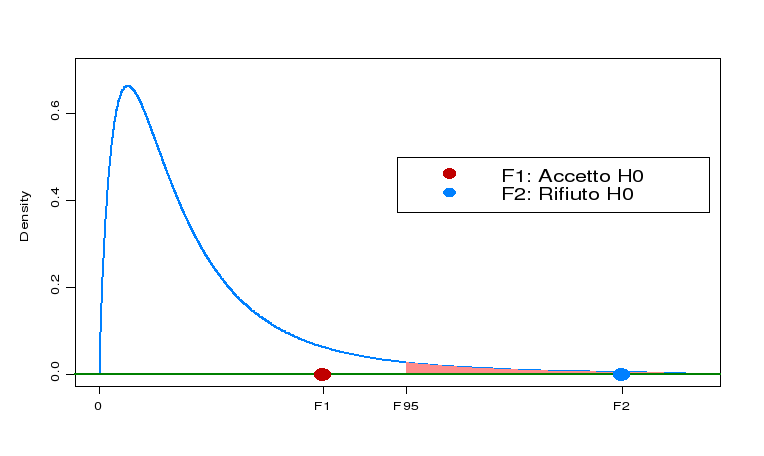
\includegraphics[scale=0.4]{5_30.png}
  \end{figure}
\end{frame}

\begin{frame}
  \vspace*{.25cm}
  The majority of the statistics packages report the result of the analysis of variance like follows:\\
  \vspace*{.5cm}
  \begin{tabular}{|c|c|c|c|c|c|}
    \hline
    & $SS$  & $df$ & $MS$  & $F$  &  $P(F)$ \\ \hline
    $Factor$  & $SS_B$  & $df_B$  &  $MS_B=\frac{SS_B}{df_B}$ &  $F=\frac{MS_B}{MS_W}$ & $P(F_{df_B,df_W}>F)$\\ \hline
    $Error$  &  $SS_W$ & $df_W$  & $MS_W=\frac{SS_W}{df_W}$  &   &   \\ \hline
    $Total$  & $SS_T$  & $df_T$  &   &   &   \\ \hline
  \end{tabular}\\
  \vspace*{.5cm}
  In conclusion, the value of real interest for the result of the analysis of variance is the \textbf{P(F)}. This value gives the criteria of choice between the null hypothesis and the alternative hypothesis according to a {\boldmath$\alpha$} value prior set.\\
  The {\boldmath$\alpha$} values commonly used are, as in all the tests, 0.05 and 0.01.
\end{frame}

\begin{frame}
  \begin{small}
    \vspace*{.25cm} 
    \textbf{Esempio}.\\
    Twelve catalytic reactions are done using three different catalysts (\textbf{levels}): A, B and C.\\
    Four reactions are assigned to each catalyst (\textbf{replications}).\\
    For each reactions, it is measured the percentage of catalysed material.\\
    \vspace*{.75cm}
    \begin{tabular}{|c|c|c|c|}
      \cline{2-4}
      \multicolumn{1}{c}{} & \multicolumn{3}{|c|}{\textbf{Catalysts}}\\ \cline{2-4}
      \multicolumn{1}{c|}{} & \hspace*{.7cm}\textbf{A}\hspace*{.7cm} & \hspace*{.7cm}\textbf{B}\hspace*{.7cm} & \hspace*{.7cm}\textbf{C}\hspace*{.7cm} \\ \hline
      \multicolumn{1}{|c|}{\hspace*{4.5cm}} & 99.2 & 99.5 & 99.3 \\ \cline{2-4}
      \multicolumn{1}{|c|}{\textbf{Percentage of catalysed}} & 99.4 & 99.4 & 99.4 \\ \cline{2-4}
      \multicolumn{1}{|c|}{\textbf{material}} & 99.3 & 99.2 & 99.5 \\ \cline{2-4}
      \multicolumn{1}{|c|}{} & 99.1 & 99.1 & 99.3 \\ \hline
      \multicolumn{1}{|c|}{\textbf{Mean of treatments}} & \textbf{99.250} & \textbf{99.300} & \textbf{99.375} \\ \hline
      \multicolumn{1}{|c|}{\textbf{Total mean}} & \multicolumn{3}{|c|}{\textbf{99.308}} \\ \hline 
    \end{tabular}\\
    \vspace*{.5cm}
  \end{small}
\end{frame}

\begin{frame}
  \begin{small}
    \vspace*{.25cm} 
    The calculated mean within the three subgroups do not seem to be especially different among them.\\
    The analysis of variance table (ANOVA Table) results to be:\\
    \vspace*{.5cm}
    \hspace*{.75cm}
    \begin{tabular}{|c|c|c|c|c|c|}
      \cline{2-6}
      \multicolumn{1}{c|}{\hspace*{3.5cm}}  & \textbf{SS}  & \textbf{df} & \textbf{MS}  & \textbf{F}  &  \textbf{P(F)} \\ \hline
      \textbf{Catalysts}  & 0.032  & 2  &  0.016 &  0.802 & 0.478 \\ \hline
      \textbf{Residuals}  &  0.177 & 9  & 0.020  &   &   \\ \hline
      \textbf{Total}  & 0.209  & 11  &   &   &   \\ \hline
    \end{tabular}\\
    \vspace*{.5cm}
    As $ P(F) = P(F_{2, 9} > 0.802) = 0.478 $ we can accept the null hypothesis for the confidence level  {\boldmath$1-\alpha$}, with {\boldmath$\alpha$} equal both to 0.05 and 0.01.\\
    \vspace*{.25cm}
    Or rather, the means, calculated within the subgroups (according to the catalysts) are not very different among them. As consequence, it has no influence on the variable answer (percentage of catalysed material) to use the catalysts A, B or C  .
  \end{small}
\end{frame}

\livelloB{Mathematical formulation}

\begin{frame}
  \vspace*{.25cm} 
  \textbf{The analysis of variance is based on the additive effects of the factors that have been taken into consideration}. In the easiest model, that only considers one factor at two or more levels, every single observation {\boldmath$X_{ij}$} can be written as
  $$ X_{ij} = \mu + \alpha_j + \varepsilon_{ij} $$\\
  \vspace*{.15cm}
  as it is determined:
  \begin{itemize}
    \item by \textbf{the overall mean} {\boldmath$\mu$} that defines the size of the experiment;
    \item by \textbf{the factor} {\boldmath$\alpha_j$} \textbf{of the treatment} $ j $th;
    \item by a \textbf{random factor}  {\boldmath$\varepsilon_{ij}$} called \textbf{residual} or \textbf{experimental error}.
  \end{itemize}
\end{frame}

\begin{frame}
  It is important to remember that \textbf{error} is not synonym for mistake, but \textbf{it shows the effect of a variety of unknown phenomenon, not valuated or not checked} in the experiment.\\ 
  In this model, the \textbf{effect} {\boldmath$\alpha$} \textbf{of the treatment} is measured as:
  $$ \alpha_j = \mu_j - \mu $$
  where {\boldmath$\mu_j$} is the mean of the treatment $ j $th and {\boldmath$\mu$} is the overall mean, and where $ \varepsilon_{ij} \in \varepsilon \sim N(0,\sigma_\varepsilon) $.\\
  In other words, the residuals of the model are distributed with null mean and constant variance, independently of the $ j $ group they belong to and of the $ i $ observation taken into consideration.\\
  The normality condition of the residual of the model is the validity condition of the model itself.
\end{frame}

\begin{frame}
  \vspace*{.25cm} 
  In descriptive terms, a similar formulation of the analysis of variance model implies that every observation is the result:\\
  \begin{itemize}
    \item of the population overall mean ($ \mu $),
    \item more an effect that comes from the treatment ($ \alpha_j $),
    \item more a random effect independent of the treatment ($ \varepsilon_{ij} $).
  \end{itemize}
  \vspace*{.25cm}
  If the third condition is not checked, another systematic effect (not random) arises in the model beyond the treatment taken into consideration. \\
  \vspace*{.25cm} 
  In other words, the difference among the means, calculated within the subgroups, is not explicable by that specific model, or rather, that model is not suitable to explain the data taken into consideration.
\end{frame}

\begin{frame}
  \vspace*{.25cm} 
  Going from the theoretical enunciation to the experimental data, it is possible to write that every single data {\boldmath$X_{ij}$} of a specific treatment is given by
  $$ X_{ij} = \overline{\overline{X}}+a_j+e_{ij} \mbox{,} $$
  with
  $$ a_j = \overline{X}_j - \overline{\overline{X}} \mbox{,} $$
  where:
  \begin{itemize}
    \item $ \overline{\overline{X}} $ is the overall mean;
    \item $ a_j $ is the effect of the treatment $ j $; 
    \item $e_{ij} $ indicates the unknown factors.
  \end{itemize}
\end{frame}

\begin{frame}
  \begin{small}
    \vspace*{.25cm} 
    \ It is clear that:
    \begin{itemize}
      \item The overall mean {\boldmath $ \overline{\overline{X}} $}, calculated on the sample, represents an estimation of the population mean {\boldmath $ \mu $};
      \item the effect of the treatment $a_j$ represents an estimation of the $ j $th treatment {\boldmath $ \alpha_j $};
      \item the {\boldmath $ e_{ij} $} values, in order for the model to be considered valid, have to be considered as a random sample of the population of the $\varepsilon$;
    \end{itemize}
    As consequence, the analysis of variance is valid if, and only if, the empirical residuals can be considered as a sample from a normal population. \\
    Graphic tools, as the normal probability plot or statistical tests such as the Anderson Darling test to check the normality, applied to the residuals series, are compulsory for the model validation.
  \end{small}
\end{frame}

\begin{frame}
  \vspace*{.25cm} 
  The assumptions of validity of the analysis of variance depend on the error {\boldmath$e_{ij}$} that:
  \begin{itemize}
    \item must be independent among them;
    \item must be normally distributed.
  \end{itemize}
  \vspace*{.25cm}
  Moreover, the variances of the various groups must be homogeneous. \\
  \vspace*{.5cm}
  The reasons why the validation of the conditions at the basis of the model are made after the estimation of the model itself, are practice and not methodological.\\
  \vspace*{.5cm}
  The advantage of this approach will be clear when we will show models of analysis of variance with more than one factor.
\end{frame}

\livelloB{The contrasts}

\begin{frame}
  \vspace*{.75cm}
  When the null hypothesis is refused, a further research to \textbf{highlight which of the relative means of the various treatments are significantly different} is carried on.\\
  \vspace*{.75cm}
  In order to do that \textbf{the multiple comparison method} is used; these comparisons can be:
  \begin{itemize}
    \item simples, or rather conducted on couple of single treatments;
    \item complexes, or rather among groups of treatments.
  \end{itemize}
\end{frame}

\begin{frame}
  \vspace*{.75cm}
  The \textbf{multiple comparison analysis} can be seen as an in-depth analysis of the ANOVA because it allows the factorization of the variance among the treatments. This method has some advantages:
  \vspace*{.50cm}
  \begin{itemize}
    \item it uses all the data;
    \item it uses the residual variance to evaluate the error;
    \item does not decrease the value {\boldmath $ \alpha $} for each of the possible comparison.
  \end{itemize}
  \vspace*{.75cm}
  A great number of multiple comparison method uses the \textbf{contrasts}.\\
\end{frame}

\begin{frame}
  \vspace*{.25cm}
  The contrasts are linear combination of the factors' mean:
  $$ C = \sum_{j=1}^p{c_j\overline{x}_j} \mbox{.} $$
  The sum of the contrasts has to be equal to zero:
  $$ \sum_{j=1}^p{c_j} = 0 \mbox{.} $$ \\
  \vspace*{.5cm}
  In a described system with $ p $ factors, $ p-1 $ independent contrasts are possible, each of them with $ 1 $ df.\\
\end{frame}

\begin{frame}
  \vspace{.50cm}
  The deviance of each contrast is given by:
  $$ SS_C = \frac{(\sum_{j=1}^p{c_j\overline{x}_j})^2}{n\sum_{j=1}^p{c_j^2}} $$
  with just one degree of freedom.\\
  \vspace*{.25cm}
  As we have just said, $ df_C = 1 $ then $ MS_C = SS_C $.\\
  \vspace*{.50cm}
  The significance of a contrast is obtained dividing its $MS_C$ by $MS_W$:
  $$ F = \frac{MS_C}{MS_W}\sim F_{1,\,n-p} \mbox{.} $$
\end{frame}

\begin{frame}
  The \textbf{orthogonal contrasts} are one of the most important kind of contrast.\\
  Two contrasts are defined as orthogonal when the sum of their coefficients, respectively $c_j$ and $d_j$, is equal to zero:
  $$ \sum_{j=1}^p{c_jd_j} = 0 \mbox{;} $$
  where $ d_j $ e $ c_j $ are the orthogonal among themselves coefficients.\\ 
  \vspace{0.25cm}
  In other words, two contrasts are orthogonal if they are equal to zero:
  \begin{itemize}
    \item the sum of the coefficients by row;
    \item the sum of the coefficients by column.\\
  \end{itemize}
  \vspace{0.5cm}
  Two orthogonal contrasts are also independent.
\end{frame}

\begin{frame}
  \vspace{.5cm}
  \textbf{Example}.\\
  \vspace*{.5cm}
  It is carried an experiment to test two different treatments $A_1$ e $A_2$. It is added a checking group, $C$ to the two treatments.\\
  \vspace*{.5cm}
  The F test results to be significant. It is highlighted a difference among the three treatments. In this case the contrasts' coefficients analysis is carried in order to evaluate which are the significant differences.\\
  \vspace*{.5cm}
  The most logical factorization of the problem is the following one:
  \begin{itemize}
    \item comparison among the checking group $ C $ and the two treatments $ (A_1+A_2) $;
    \item comparison between the two treatments $ A_1 $ and $ A_2 $.
  \end{itemize}
\end{frame}

\begin{frame}
  \vspace*{.75cm}
  \begin{itemize}
    \item In the first comparison, $C$ vs $A_1+A_2$, it wants to be checked the null hypothesis
    $$ H_0:\,\mu_c-\frac{\mu_{A1}+\mu_{A2}}{2} = 0 $$
    from it, it is possible to obtain the coefficients $(+1\;-\frac{1}{2}\;-\frac{1}{2})$ or, that is the same, the coefficients $ (+2 \; -1 \; -1) $\\
    \vspace*{.75cm}
    \item In the second comparison, $A_1$ vs $A_2$, the null hypothesis is checked
    $$ H_0:\,\mu_{A1}-\mu_{A2} = 0 $$
    and from it it is possible to obtain the coefficients $(0\;+1\;-1)$
  \end{itemize}
\end{frame}

\begin{frame}
  \vspace{.25cm}
  The table that follows shows the comparison coefficients in the whole form\\
  \vspace{.25cm}
  \hspace{.75cm}
  \begin{tabular}{|c|c|c|c|c c|}
    \cline{2-6}
    \multicolumn{1}{c|}{\hspace*{3.5cm}}  & $ C $  & $ A1 $ & $ A2 $ & \textbf{Sum per line} & \\ \hline
                    $C$ against $A_1+A_2$  & $ +2 $ & $ -1 $ & $ -1 $ & $ 0 $                   & \\ \hline
                      $A_1$ against $A_2$  & $ 0 $  & $ +1 $ & $ -1 $ & $ 0 $                   & \\ \hline
                    Products per column  & $ 0 $  & $ -1 $ & $ +1 $ & $ 0 $                   & \\ \hline
                 \textbf{Total column}  & $ 0 $  & $ -1 $ & $ +1 $ & $ 0 $                   & \\ \hline
  \end{tabular}\\
  \vspace{0.2cm}
  The comparisons, formulated in this way, respect all the orthogonality conditions.\\
  \vspace{.20cm}
  \begin{itemize}
    \item The comparison of $C$ against $A_1+A_2$ allows us to verify if the check has different effects compared to the two treatments, linked in only one group;
    \item The comparison of $A_1$ against $A_2$ allows us to highlight if the two treatments lead to different effects among them.  
  \end{itemize}
\end{frame}

\livelloB{Comparison with t test with two independent samples}

\begin{frame}
  \vspace*{.5cm} 
  The analysis of variance can be also applied to an experiment with only one factor (treatment) and two levels. For this case, the Student's t method has been already presented.\\
  \vspace*{.5cm}
  In reality, t test and F test are two methods that are only apparently different to carry the same analysis:  \textbf{the t test can be seen as a special case of the analysis of variance}, applied to only two groups or, to better say, \textbf{the analysis of variance is the extention of the Student's t with bilateral alternative hypothesis to more groups and with more factors}.
\end{frame}

\begin{frame}
  \vspace*{.25cm} 
  In the case of one factor with two groups, between the t and F distributions, it exists a precise mathematical relation:\\
  $$ F_{(1,\nu)}=t^2_{(\nu)} \mbox{,} $$\\
  that can be written as:\\
  $$ t_{(\nu)}=\sqrt{F_{(1,\nu)}} \mbox{;} $$\\
  where $ \nu $ is the number of the degrees of freedom. \\
  \vspace*{.25cm}
  \textbf{The F value with 1 and {\boldmath $ \nu $} degrees of freedom is equal to the square of t with {\boldmath $ \nu $} degrees of freedom.}\\
  \vspace*{.25cm}
\textbf{The two distributions of the critical values for the same probability {\boldmath $ \alpha $} are equivalent.}
\end{frame}



\livelloA{Two or more factors analysis of variance}

\begin{frame}
  \begin{footnotesize}
    In the case of the experiment with two factors, the collected data can be represented in a two-dimensions table: \\
    \vspace*{.25cm} 
    \hspace*{.7cm}
    \begin{tabular}{|c|c|c|c|c|}
      \cline{2-5}
      \multicolumn{1}{c}{} & \multicolumn{4}{|c|}{\textbf{Factor A}}\\ \hline
      \hspace*{.2cm}\textbf{Factor}\hspace*{.2cm} & $A_1$ & $A_2$ & $A_3$ & Means\\ 
      \textbf{B} &  &  &  &    \\ \hline
      & $x_{111},x_{211},$\hspace*{.7cm} & $x_{112},x_{212},$\hspace*{.7cm} & $x_{113},x_{213},$\hspace*{.7cm} & \\
      $B_1$ & $x_{311},x_{411}$\hspace*{.7cm} & $x_{312},x_{412}$\hspace*{.7cm} & $x_{313},x_{413}$\hspace*{.7cm} & $\overline{\overline{X}}_{1.}$\\ 
      & \multicolumn{1}{|r|}{$\overline{X}_{11}$} & \multicolumn{1}{|r|}{$\overline{X}_{12}$} & \multicolumn{1}{|r|}{$\overline{X}_{13}$} &  \\ \hline
      & $x_{121},x_{221},$\hspace*{.7cm} & $x_{122},x_{222},$\hspace*{.7cm} & $x_{123},x_{223},$\hspace*{.7cm} & \\
      $B_2$ & $x_{321},x_{421}$\hspace*{.7cm} & $x_{322},x_{422}$\hspace*{.7cm} & $x_{323},x_{423}$\hspace*{.7cm} & $\overline{\overline{X}}_{2.}$\\ 
      & \multicolumn{1}{|r|}{$\overline{X}_{21}$} & \multicolumn{1}{|r|}{$\overline{X}_{22}$} & \multicolumn{1}{|r|}{$\overline{X}_{23}$} &  \\ \hline
     	& &  &  & \\
	Means & $\overline{\overline{X}}_{.1}$ & $\overline{\overline{X}}_{.2}$ & $\overline{\overline{X}}_{.3}$ & $\overline{\overline{\overline{X}}}$\\ 
	&  &  &  &  \\ \hline
    \end{tabular}   
    \vspace*{.5cm}
  \end{footnotesize}                                                                                                   
\end{frame}

\begin{frame}
  \vspace*{.25cm} 
  In this case there are three null hypothesis that have to be checked against as much alternative hypothesis.\\
  \vspace*{.5cm}
  The first hypothesis regards the effect of the factor (A) on the answer variable:
  $$ H_0: \,\mu_{.1} = \mu_{.2} = \dots = \mu_{.p} $$
  $$ H_A: \, \exists i,j \mid \mu_{.i} \neq \mu_{.j}\;\;\;(i,\,j=1,\,\dots,\,p) $$
  where $ p $ is the number of levels of the factor (A).\\
  \vspace*{.75cm}
  Or rather, the factor (A), indipendentently of the factor (B), has no effect on the answer variable.
\end{frame}

\begin{frame}
  \vspace*{.25cm} 
  The second hypothesis regards the effect of the factor (B) on the answer variable:
  $$ H_0:\,\mu_{1.}=\mu_{2.}=\dots=\mu_{q.} $$
  $$ H_{A}:\,\exists i,j\mid\mu_{i.}\neq\mu_{j.}\;\;\;(i,\,j=1,\,\dots,\,q) $$
  where $ q $ is the number of levels of the factor (B).\\
  \vspace*{.75cm}
  Or rather, the factor (B), indipendently of the factor (A), has no effect on the answer variable.\\
  \vspace*{.5cm}
  The first two hypothesis can be considered as two independent analysis of variance with a single factor.
\end{frame}

\begin{frame}
  \begin{small}
    The third hypothesis regards the combined effect of the treatments A and B on the answer variable. The combined effect is defined \textbf{interaction}.\\
    \vspace*{.2cm}
    \textbf{Example}. In a catalytic reaction there are:
    \begin{itemize}
      \item a positive effect (or rather an \textbf{increase} of the percentage of catalytised material) going from a temperature of $140^\circ C$ to a temperature of $180^\circ C$ using the catalyst {\boldmath$C_1$};
      \vspace*{.2cm}
      \item a negative effect (or rather a \textbf{decrease} of the percentage of catalysed material)  going from a temperature of $140^\circ C$ to a temperature of $180^\circ C$ using the catalyst {\boldmath$C_2$};
    \end{itemize}
    \vspace*{.2cm}
    As the algebra that regards the interactions is relatively more complex than the algebra of principal effects, we will avoid to delve into this topic.\\
    \vspace*{.2cm}
    It is enough to remember that, in a two or more factors analysis of variance, it exists also a component that regards the interaction.
  \end{small}
\end{frame}

\livelloB{Deviance, degrees of freedom and variance}

\begin{frame}
  \vspace*{.25cm} 
  The \textbf{total deviance} or {\boldmath$SS_{Total}$} (Total Sum of Squares) defines the residual sum of squares of every value of the overall mean.
  $$ SS_{Total} = \sum_{k=1}^q \sum_{j=1}^p \sum_{i=1}^{n}{(X_{ijk}-\overline{\overline{\overline{X}}})^2} $$ \\
  \vspace{-0.3cm}
  where:\\
  \vspace{-0.3cm}
  \begin{itemize}
    \item $ X_{ijk} $ is the $ i $th observation that regards the $ j $th level of the first factor and the $ k $th level of the second factor;
    \item $ n $ is the size (considered constant) of the corresponding group of observations at the $ j $th level of the first factor and at the $ k $th level of the second factor;
    \item $ p $ is the number of levels for the first factor;
    \item $ q $ is the number of levels for the second factor.
  \end{itemize}
  The {\boldmath$SS_{Total}$} defines the total variability of the sample.\\
\end{frame}

\begin{frame}
  The \textbf{deviance between treatments} or {\boldmath$SS_{\,Between}$} (Between Sum of Squares) defines the residuals sum of the squares of every group mean from the overall mean, multiplied the number of data of the corresponding group.  It exists three components ``between'': one for the factor A, one for the factor B and one for the interaction.\\
  The calculation of the component ``between'' is really similar to the calculation of the one-factor analysis of variance.\\
  $$ SS_A = qn \sum_{j=1}^p{(\overline{\overline{X}}_{j.}-\overline{\overline{\overline{X}}})^2}\mbox{\hspace*{2.75cm}For the factor  (A).} $$
  $$ SS_B = pn \sum_{k=1}^q{(\overline{\overline{X}}_{.k}-\overline{\overline{\overline{X}}})^2}\mbox{\hspace*{2.75cm}For the factor (B).} $$
  $$ SS_{AB} = n \sum_{j=1}^p{\sum_{k=1}^q{(\overline{X}_{jk}-\overline{\overline{X}}_{j.}-\overline{\overline{X}}_{.k}+\overline{\overline{\overline{X}}})^2}}\mbox{\hspace*{.6cm}For the interaction (AB).} $$
\end{frame}

\begin{frame}
  \vspace*{.25cm} 
  The {\boldmath$SS_{\,Between}$} defines the variability among groups independently of the dispersion of the single observations within each group.\\
  \vspace*{.5cm} 
  The \textbf{deviance within treatments} or {\boldmath$SS_{\,Within}$} (Within Sum of Squares), also called \textbf{error}, defines the residuals sum of squares of every value of the mean of its group.\\
  $$ SS_{\,Within}=\sum_{k=1}^{q} \sum_{j=1}^{p} \sum_{i=1}^{n}{(X_{ijk}-\overline{X}_{jk})^2} $$\\
  \vspace*{.25cm}
  The {\boldmath$SS_{\,Within}$} defines the variability within single groups independently of the position of the group compared to/around the central mean of the sample or compared to/around the mean calculated for a single factor. 
\end{frame}

\begin{frame}
  \vspace*{.75cm} 
  As the remaining part of the variability quota does not represent only the sum of the squares within the groups but also the errors sum of squars, in the future it will be preferable to use {\boldmath$SS_{E}$} instead of {\boldmath$SS_{\,Within}$} or {\boldmath$SS_{W}$}.\\
  \vspace*{.5cm} 
  Similarly, the corresponding degrees of freedom will be indicated with $ df_{E} $ and the ratio between the sum of squares and the degrees of freedom with $ MS_{E} $.
\end{frame}

\begin{frame}
  \vspace*{.25cm}
  It is possible to demonstrate, also in this case, that
  $$ SS_{\,Total}=SS_{\,Between}+SS_{E} $$
  where
  $$ SS_{\,Between}=SS_A+SS_B+SS_{AB} $$
  with
  \begin{itemize}
    \item $SS_A$: sum of squares attributable to the factor (A);
    \item $SS_B$: sum of squares attributable to the factor (B);
    \item $SS_{AB}$: sum of squares attributable to the interaction between (A) and (B).
  \end{itemize}	
\end{frame}

\begin{frame}
  Starting from the sum of squares \textbf{SS}, it is possible to calculate the means of squares \textbf{MS} dividing by the appropriate degrees of freedom.\\
  \vspace*{.15cm}
  The calculation of the degrees of freedom still results to be quite easy.\\
  \begin{itemize}
    \item The degrees of freedom of each factor are equal to the number of levels of that factor minus one.
    \item The degrees of freedom of the interaction between the two factors are given by the product of the degrees of freedom of each factor.
    \item The degrees of freedom of the residuals are equal to the product of the number of groups and the number of observations within each group minus one. In other words, they are equal to the number of observations minus one and minus the sum of the degrees of freedom of each factor and the interaction.
  \end{itemize}
  As in the univariate case, it is valid the following relation:
  $$ df_{Total}=df_A+ df_B+df_{AB}+df_{E} \mbox{.} $$
\end{frame}

\begin{frame}
  \textbf{Example}. It is supposed to carry out an experiment with two factors, (A) and (B), where:
  \begin{itemize}
    \item the factor (A) has  two levels;
    \item the factor (B) has three levels;
    \item each combinations of factors' levels has four replications.\\
  \end{itemize}
  \vspace{0.25cm}
  It follows that:
  \begin{itemize}
    \begin{small}
    \item the total number of observations $ N $ is equal to $ 2 \cdot 3 \cdot 4 = 24 $ from which {\boldmath$ df_T = 23 $};\\
    \item the factor (A) has two levels, from which {\boldmath$df_A=1$};\\
    \item the factor (B) has three levels, from which {\boldmath$df_B=2$};\\
    \item the interaction (AB) has degrees of freedom {\boldmath$df_{AB}=df_A\cdot df_B=2$};\\
    \item the residual (error) has degrees of freedom equal to 6 (groups) multiplied by 3 (number of observations within each group minus one), that is {\boldmath$df_E=6\cdot 3=18$}.\\
    \end{small}
  \end{itemize}
\end{frame}

\begin{frame}
  \vspace*{.25cm} 
  Starting from the \textbf{SS} it is possible to calculate the means of squares MS:\\
  \vspace*{.25cm}
  $$ MS_A=\frac{SS_A}{df_A} $$\\
  \vspace*{.25cm}
  $$ MS_B=\frac{SS_B}{df_B} $$\\
  \vspace*{.25cm}
  $$ MS_{AB}=\frac{SS_{AB}}{df_{AB}} $$\\
  \vspace*{.25cm}
  $$ MS_E=\frac{SS_E}{df_E} $$\\
\end{frame}

\begin{frame}
  \vspace*{.25cm} 
  The {\boldmath$MS_A$}, {\boldmath$MS_B$} and {\boldmath$MS_{AB}$} , if the null hypothesis are true, or rather if the factors (A) and (B) do not have any effects on the answer variable, they are all independent estimations of the variance of $\sigma^2_\varepsilon$ from which the sample has been extracted.\\
  \vspace*{.5cm}
  {\boldmath$MS_E$} is an estimation of $\sigma^2_\varepsilon$.\\
  \vspace*{.5cm}
  As consequence, if all the hypothesis $H_0$ are valid:\\
  \vspace*{.25cm}
  $$ \frac{MS_A}{\sigma^2_A}=\frac{MS_A}{\sigma^2_\varepsilon}\sim\chi^2_{df_A}\mbox{\hspace*{1cm}}\frac{MS_B}{\sigma^2_B}=\frac{MS_B}{\sigma^2_\varepsilon}\sim\chi^2_{df_B} $$\\
  \vspace*{.25cm}
  $$ \frac{MS_{AB}}{\sigma^2_{AB}}=\frac{MS_{AB}}{\sigma^2_\varepsilon}\sim\chi^2_{df_{AB}}\mbox{\hspace*{1cm}}\frac{MS_E}{\sigma^2_E}=\frac{MS_E}{\sigma^2_\varepsilon}\sim\chi^2_{df_E} $$
  \setlength{\unitlength}{.5cm}
  \begin{picture}(50,3)
    \put(17,4.4){\oval(9,3)}
  \end{picture}
\end{frame}

\begin{frame}
  \vspace*{.5cm} 
  and, as consequence, the ratios
  $$ F_A=\frac{MS_A}{MS_E}\sim F_{df_A,df_E}\mbox{\hspace*{1.5cm}} F_B=\frac{MS_B}{MS_E}\sim F_{df_B,df_E} $$\\
  \vspace*{.5cm}
  $$ F_{AB}=\frac{MS_{AB}}{MS_E}\sim F_{df_{AB},df_E} $$\\
  \vspace*{.5cm}
  tend to be distributed as a \textbf{F of Fisher-Snedecor} with appropriate degrees of freedom.
\end{frame}

\begin{frame}
  \vspace*{.25cm} 
  It is then possible to build a table of the analysis of variance like follows:\\
  \vspace*{.75cm}
  \begin{tabular}{|c|c|c|c|c|c|}
    \hline
    & SS & df & MS & F & P(F)\\ \hline
    A & $SS_A$ & $df_A$ & $MS_A=\frac{SS_A}{df_A}$  & $\frac{MS_A}{MS_E}$ & $P(F_{df_A,df_E}>F)$\\ \hline
    B & $SS_B$ & $df_B$ & $MS_B=\frac{SS_B}{df_B}$  & $\frac{MS_B}{MS_E}$ & $P(F_{df_B,df_E}>F)$\\ \hline
    AB & $SS_{AB}$ & $df_{AB}$ & $MS_{AB}=\frac{SS_{AB}}{df_{AB}}$  & $\frac{MS_{AB}}{MS_E}$ & $P(F_{df_{AB},df_E}>F)$\\ \hline
    \textit{Error} & $SS_E$ & $df_E$ & $MS_E=\frac{SS_E}{df_E}$  &  & \\ \hline
    \textit{Total} & $SS_T$ & $df_T$ &   &  & \\ \hline
  \end{tabular}   
  \vspace*{.5cm}      
\end{frame}

\begin{frame}
  \vspace*{.25cm} 
  The rules to read this table are identical to those of one-factor case.\\
  \vspace*{.25cm} 
  The different concept is that, in a multivariate case, there are a lot of null hypothesis that have to be checked.\\
  \vspace*{.5cm} 
  \textbf{Example}.\\
  An experiment with three factors (A, B, C) requires the calculation of eight MS, or rather: A, B, C, AB, AC, BC, ABC, E.\\
  \vspace*{.25cm} 
  Assuming, for example, that the interaction ABC is not significant, it implies that this interaction can be removed from the analysis.
\end{frame}

\begin{frame}
  \vspace*{.25cm} 
  But, the equation
  $$ SS_{T}=SS_A+SS_B+SS_C+SS_{AB}+SS_{AC}+SS_{BC}+SS_{ABC}+SS_E $$
  must be always true.\\
  \vspace*{.25cm}
  If we leave ABC, the equation will not be true.\\
  \vspace*{.5cm}
  In practice, the equation is defined like follows:
  $$ SS_{T} = SS_A + SS_B + SS_C + SS_{AB} + SS_{AC} + SS_{BC} + SS_{E1} \mbox{,} $$
  where:
  $$ SS_{E1} = SS_E + SS_{ABC} \mbox{.} $$
\end{frame}

\begin{frame}
  \vspace*{.25cm} 
  The degrees of freedom have to be modified too, so that:
  $$ df_{E1}=df_E+df_{ABC} \mbox{.} $$
  If the \textbf{SS} of the error and the degrees of freedom change, it will then change also the \textbf{MS} of the error:
  $$ MS_{E1}=\frac{SS_{E1}}{df_{E1}} \mbox{.} $$\\
  \vspace*{.5cm}
  \textbf{It follows that all the ratios F and the relative probabilities are altered.}
\end{frame}

\begin{frame}
  \vspace*{.5cm} 
  In conclusion, in a multivariate ANOVA analysis, it is necessary to carry on with the estimation of the more \textbf{parsimonious} model for interactions that follows, removing one terms at a time from the analysis.\\
  \vspace*{.5cm}
  The choice of the term that has to be removed first is done according to two choice criterions:
  \begin{itemize}
    \item the degree of the term: the terms with an higher degree are removed first;
    \item with the same degree, the term with smaller F value or $ P(F) $ higher.
  \end{itemize}
  \vspace*{.5cm}
  This has to stay within hierarchical models.
\end{frame}

\livelloB{Mathematical formulation}

\begin{frame}
  \vspace*{.25cm} 
  The mathematical model formulation of the ANOVA with two or more factors result to be an easy enlargement of the univariate model, every single observation {\boldmath $ X_{ijk} $} can be written as
  $$ X_{ijk}=\mu+\alpha_{j}+\beta_{k}+\gamma_{jk}+\varepsilon_{ijk} $$
  as it is determined:
  \begin{itemize}
    \item by the \textbf{overall mean} {\boldmath$\mu$} that defines the dimension of the experiment;
    \item by the \textbf{parameter} {\boldmath$\alpha_{j}$} that regards the $ j $th \textbf{level} of the factor (A);
    \item by the \textbf{parameter} {\boldmath$\beta_{k}$} that regards the  $ k $th \textbf{level} of the factor (B);
    \item by the \textbf{parameter}  {\boldmath$\gamma_{jk}$} that regards \textbf{the interactions on the levels} $ j $th and $ k $th of the factors (A) and (B);
    \item by a \textbf{random term} {\boldmath$\varepsilon_{ijk}$} called \textbf{residual} or \textbf{experimental error}.
   \end{itemize}
\end{frame}

\begin{frame}
  \vspace*{.25cm} 
  In this case too:
  $$ \varepsilon_{ijk}\,\in\, \varepsilon \sim N(0,\,\sigma_{\varepsilon})\mbox{\hspace*{.75cm}}\forall\mbox{\hspace*{.75cm}}(i,\,j,\,k) $$
  In other words, the error term of the model is distributed with null mean and constant variance.\\
  \vspace*{.25cm}
  The normality condition of the error term of the model is one of the validity conditions of the model itself, together with the independence of the residuals values.\\
  \vspace*{.5cm}
  In conclusion, \textbf{the residuals analysis, in the multivariate case, is identical to the univariate case.}
\end{frame}


\livelloB{Types of experimental plans}

\begin{frame}
  \vspace*{.25cm}
  Basically, there are 4 types of experimental plans:
  \begin{itemize}
    \begin{small}
      \item[1.] \textbf{balanced} where $ n_{ij} $ is equal to each combination $ {ij} $, or rather, the number of data in every cell is equal;
      \vspace{.15cm}
      \item[2.] \textbf{proportional} to the number of replication of the marginals of the size table.\\
        In the two-factors case:
        $$ n_{ij}=\frac{n_in_j}{N} $$
        where:
        \begin{itemize}
          \item $ n_{ij} $ is the number of data at the crossing between the line $ i $ and the column $ j $;
          \item $ n_i $ is the total number of the observations within the line $ i $;
          \item $ n_j $ is the total number of observations within the line $ j $;
          \item $ N $ is the total number of the observations.	
        \end{itemize}
    \end{small}
  \end{itemize}
\end{frame}

\begin{frame}
  \begin{itemize}
  \item[]  \textbf{Example}. An experimental plan is composed by 4 level of the factor A and 3 levels of the factor B, as shown in the table:
    \begin{center}
      \begin{tabular}{|c|c|c|c|c|c|}
        \hline
        & $a_1$ &   $a_2$ &  $a_3$ &  $a_4$ & \textbf{Total}\\ \hline
        $b_1$ & 3 & 6 & 9 & 6 & 24\\ \hline
        $b_2$ & 4 & 8 & 12 & 8 & 32\\ \hline
        $b_3$ & 2 & 4 & 6 & 4 & 16\\ \hline
        \textbf{Total} & 9 & 18 & 27 & 18 & 72\\ \hline
      \end{tabular}
    \end{center}
    \vspace{.5cm}
    \item[3.] \textbf{not balanced} where the number of data in each cell is different and not proportional;
    \vspace{.15cm}
    \item[4.] \textbf{with empty cells}.
  \end{itemize}
\end{frame}

\livelloB{Fixed and random effects}

\begin{frame}
\vspace*{.25cm} 
In an analysis of variance a \textbf{fix effect} is a factor whose levels cover all the possible modalities of the phenomenon that the factor expresses.\\
\vspace*{.5cm} 
\textbf{Example}. In a company there are two identical measuring devices with the same duty. An experiment has to be carried out in order to understand if there is a significant difference in the way the two devices measure.\\
\vspace*{.5cm} 
As only two devices exist, a factor with two level expresses the wholeness, or rather the whole population, of the devices.\\
\vspace*{.5cm} 
In this case the factor (effect) is defined as \textbf{fix} and it is applied to a standard ANOVA (shown as \textbf{ANOVA I}).
\end{frame}

\begin{frame}
  \vspace*{.5cm} 
  \textbf{Example}.\\
  \vspace*{.5cm} 
  An oven, used for firing a certain material, has a temperature range included between $120^{\circ}C$ and $180^{\circ}C$.\\
  \vspace*{.5cm} 
  Two temperature are set up $130^{\circ}C$ and $170^{\circ}C$.\\
  \vspace*{.5cm} 
  The two temperatures represent two level \textbf{fix}: low and high temperature.\\
  \vspace*{.5cm} 
  In this case they are fixed effects too.
\end{frame}

\begin{frame}
  \vspace*{.25cm} 
  \textbf{Example}.\\
  \vspace*{.25cm} 
  A certain phase of a manufactoring process requires a measurement by an operator.\\
  \vspace*{.25cm} 
  The operators can be several and it is not possible to check whose operator will do the measurement.\\
  \vspace*{.25cm} 
  It is then carried out an experiment, using two operators, in order to test if an operator effect exists in the manufactoring process.\\
  \vspace*{.25cm} 
  The two operators are not the only two operators but a random sample of all the possible operators.\\
  \vspace*{.25cm} 
  In this case it is ANOVA with \textbf{random effects}.
\end{frame}

\begin{frame}
  \vspace*{.25cm} 
  A random effects ANOVA (usually shown as \textbf{ANOVA II}) follows the same methods of a fixed effects ANOVA analysis.\\
  \vspace*{.25cm}
  Anyway, there are some difference as regards the formulation of the hypothesis:
  $$ H_0: \; \sigma^{2}_B = 0 $$
  $$ H_A: \; \sigma^{2}_B > 0 $$
  where $\sigma^{2}_B$ is the answer variance due to the difference among treatments.\\
  \vspace{.25cm}
  This happens because it has no sense to test the single effect hypothesis as the chosen levels are \textbf{samples randomly extracted from the population}.\\
\end{frame}

\begin{frame}
  In the ANOVA II, if $ H_0 $ is refused, the multiple comparisons that have no meaning, are not done.\\
  The difference between two specific levels is not of interest because these are representative of a wider population.\\ 
  \vspace{.25cm}
  It follows that it is useful to proceed with a quantitative valuation of the variance by the calculation of the  \textbf{components of the variance}.\\
  \vspace*{.25cm}
  \begin{itemize}
    \item $MS_B$ is a correct estimator of $ \sigma^{2}_{\varepsilon}+n \sigma^{2}_{B} $\\
      \vspace*{.25cm}
      or rather $E(MS_B)=$ $\sigma^{2}_{\varepsilon}+n \sigma^{2}_{B}$\\
    \vspace*{.75cm}
    \item $MS_E$ is a correct estimator of the variance ``within'' $ \sigma^{2}_{\varepsilon} $\\ 
      \vspace*{.25cm}
      or rather $E(MS_E)$ $=\sigma^{2}_{\varepsilon}$
  \end{itemize}
\end{frame}

\begin{frame}
  \vspace*{.25cm} 
  In order to estimate the element of variance ``between'', it is used the following formula\\
  $$ \hat{\sigma}^{2}_{B}=\frac{MS_B-MS_E}{n} \mbox{.} $$\\
  \vspace*{.25cm}
  If the null hypothesis is true, or rather that it does not exist variability due to different treatments that have been randomly chosen, then:
  $$ \sigma^{2}_{B}=0 $$ 
  $$ E(MS_B)=\sigma^{2}_{\varepsilon} $$ \\
  \vspace*{.25cm}
  And then, similarly to the fixed effects case:
  $$ F=\dfrac{\frac{MS_B}{\sigma^{2}_{\varepsilon}}}{\frac{MS_E}{\sigma^{2}_{\varepsilon}}}=\frac{MS_B}{MS_E}\sim F_{p-1,n-p} $$
\end{frame}

\begin{frame}
  If the model is not balanced, ${n}$ has to be corrected:\\
  $$ \hat{n}=\overline{n}-\frac{\sum{({n}_{i}-\overline{n})^2}}{(k-1)N} \mbox{,} $$\\
  where
  \begin{itemize}
    \item $\overline{n}$ is the mean number of data in the levels; 
    \item ${n}_{i}$ is the number of data within the level $i$;
    \item ${k}$ is the number of levels;
    \item ${N}$ is the total number of data.
  \end{itemize}
  \vspace{.50cm}
  In the case of a multifactorial ANOVA, the calculation of F ratio is modified, but the basic logic does not change.
\end{frame}

\begin{frame}
  \vspace*{.75cm}
  In conclusion, a third type of analysis exists (it will be shown as \textbf{ANOVA III}), given be the \textbf{mix of fixed and random factors}.\\
  \vspace* {.75cm}
  The hypothesis for the calculation of the ratios for the F test are equal to that we have already seen for ANOVA I and ANOVA II, even though the ratios themselves change compared to these two.
\end{frame}

\livelloB{Nested ANOVA}

\begin{frame}
  \vspace*{.25cm} 
  The analysis of variance, as it has been presented till now, assumes that, during the experiment, every level of each factor cuts across with all the levels of the other factors.\\
  \vspace*{.5cm} 
  If the number of times that a level of a factor meets all the levels of the others factors is constant for all the levels combinations, then the experiment is called \textbf{crossed} \textbf{balanced}.\\
  \vspace*{.5cm} 
  If, instead, the same number is not equal for all the combinations, then the experiment is called \textbf{crossed} \textbf{not balanced}.\\
  \vspace*{.5cm} 
  Another type of experiment is defined as \textbf{nested experiment}.
\end{frame}

\begin{frame}
  \begin{small}
    \textbf{Example}.\\
    \vspace{.15cm}
    The same pharmaceutical product is produced by two companies: A e B.\\
    \vspace{.15cm}
    The company A produces three lots of product with different concentrations $C_{A1}$, $C_{A2}$ e $C_{A3}$.\\
    \vspace{.15cm}
    The company B produces three lots of product with different concentrations $C_{B1}$, $C_{B2}$ e $C_{B3}$.\\
    \vspace{.15cm}
    For each company, two sample revelations for each concentration have to be taken into consideration.\\
    \vspace{.15cm}
    The situation can be summed up in the following diagram:\\
    \vspace{-.3cm}
  \end{small}
  \setlength{\unitlength}{.5cm}
  \begin{picture}(50,10)
    \put(5,8){A}
    \put(18,8){B}
    \put(4.75,7.75){\vector(-2,-1){2}}
    \put(5.25,7.75){\vector(0,-1){1}}
    \put(5.75,7.75){\vector(2,-1){2}}
    \put(17.75,7.75){\vector(-2,-1){2}}
    \put(18.25,7.75){\vector(0,-1){1}}
    \put(18.75,7.75){\vector(2,-1){2}}
    \put(2,5.75){$C_{A_1}$}
    \put(5,5.75){$C_{A_2}$}
    \put(8,5.75){$C_{A_3}$}
    \put(15,5.75){$C_{B_1}$}
    \put(18,5.75){$C_{B_2}$}
    \put(21,5.75){$C_{B_3}$}
    \put(2,5.5){\vector(-1,-2){.5}}
    \put(2.75,5.5){\vector(1,-2){.5}}
    \put(5,5.5){\vector(-1,-2){.5}}
    \put(5.75,5.5){\vector(1,-2){.5}}
    \put(8,5.5){\vector(-1,-2){.5}}
    \put(8.75,5.5){\vector(1,-2){.5}}
    \put(15,5.5){\vector(-1,-2){.5}}
    \put(15.75,5.5){\vector(1,-2){.5}}
    \put(18,5.5){\vector(-1,-2){.5}}
    \put(18.75,5.5){\vector(1,-2){.5}}
    \put(21,5.5){\vector(-1,-2){.5}}
    \put(21.75,5.5){\vector(1,-2){.5}}
    \put(.75,3.75){\begin{small}$R_{A_{11}}$\end{small}}
    \put(2.3,3.75){\begin{small}$R_{A_{12}}$\end{small}}
    \put(4,3.75){\begin{small}$R_{A_{21}}$\end{small}}
    \put(5.5,3.75){\begin{small}$R_{A_{22}}$\end{small}}
    \put(7.2,3.75){\begin{small}$R_{A_{31}}$\end{small}}
    \put(9,3.75){\begin{small}$R_{A_{32}}$\end{small}}
    \put(13.75,3.75){\begin{small}$R_{A_{11}}$\end{small}}
    \put(15.3,3.75){\begin{small}$R_{A_{12}}$\end{small}}
    \put(17,3.75){\begin{small}$R_{A_{21}}$\end{small}}
    \put(18.5,3.75){\begin{small}$R_{A_{22}}$\end{small}}
   \put(20.2,3.75){\begin{small}$R_{A_{31}}$\end{small}}
   \put(22,3.75){\begin{small}$R_{A_{32}}$\end{small}}
  \end{picture}
\end{frame}

\begin{frame}
  For the analysis of this type of experiment it is necessary to use a \textbf{hierarchical or nested classification} for factor, commonly known as \textbf{nested anova}.\\
  \vspace*{.5cm} 
  The attention goes on the difference between the product lots within (nested) the company.\\
  \vspace*{.5cm}
  In other words, it wants to be checked if there is a statistically significant difference between two (or more) lots, once that the company effect has been removed.\\
  \vspace*{.5cm}
  A similar case corresponds to a statistical model like:
  $$ X_{ijk}=\mu+\alpha_k+\beta_{j(k)}+\varepsilon_{i(jk)} $$
\end{frame}

\begin{frame}
  where:
  \begin{itemize}
    \item $\mu$ is the overall mean;
    \vspace*{.25cm} 
    \item $\alpha_{k}$ is the $ k $th effect of the company factor ($ \alpha $);
    \vspace*{.25cm} 
    \item $\beta_{j(k)}$ is the $ j $th effect of the lot effect ($ \beta $) nested in the $ k $th level of the company factor ($ \alpha $); %\\
    \vspace*{.25cm} 
    \item $\varepsilon_{i(jk)}$ is the $ i $th error nested in the $ j $th level of the lot factor ($ \beta $) which is nested in the $ k $th level of the company factor ($\alpha$). %\\
  \end{itemize}
  \vspace*{.25cm} 
  Two important notions are implicit:
  \begin{itemize}
    \item \textbf{the higher level affects the lower level};
    \item \textbf{the lower level has importance if it is analysed within the higher}.
  \end{itemize}
\end{frame}

\begin{frame}
  The calculation of the \textbf{SS} and the \textbf{MS} is made similarly to the formulations used in the case of crossed experiments.\\
  \vspace*{.25cm}
  In a similar case, with fixed effects, it is possible to build a table of the analysis of variance like:\\
  \vspace*{.75cm}
  \begin{tabular}{|c|c|c|c|c|c|}
    \hline
    & SS & df & MS & F & P(F)\\ \hline
    A & $SS_A$ & $df_A$ & $MS_A=\frac{SS_A}{df_A}$  & $\frac{MS_A}{MS_E}$ & $P(F_{df_A,df_E}>F)$\\ \hline
    B & $SS_B$ & $df_B$ & $MS_B=\frac{SS_B}{df_B}$  & $\frac{MS_B}{MS_E}$ & $P(F_{df_B,df_E}>F)$\\ \hline
    AB & $SS_{AB}$ & $df_{AB}$ & $MS_{AB}=\frac{SS_{AB}}{df_{AB}}$  & $\frac{MS_{AB}}{MS_E}$ & $P(F_{df_{AB},df_E}>F)$\\ \hline
    \textit{Error} & $SS_E$ & $df_E$ & $MS_E=\frac{SS_E}{df_E}$  &  & \\ \hline
    \textit{Total} & $SS_T$ & $df_T$ &   &  & \\ \hline
  \end{tabular}   
  \vspace*{.5cm}      
  \setlength{\unitlength}{.5cm}
  \begin{picture}(50,3)
    \put(19,9.5){\oval(10,1.5)}
  \end{picture}
\end{frame}

\begin{frame}
  \vspace{.25cm}
  In the nested experiments, the effects can be fixed or radom, which want different hypothesis formulations.\\
  \vspace{.25cm}
  As consequence, also the analysis of variance of nested experiments can be divided in:
  \begin{itemize}
    \item NESTED ANOVA I, where all the factors are fixed;
    \item NESTED ANOVA II, where all the factors are random;
    \item NESTED ANOVA III, where some factors are fixed and other random, usually that of lower levels.
  \end{itemize}
  \vspace{.25cm}
  The choice of the type of ANOVA and of the type of hypothesis to test depends on the formulation of the problem.\\
  \vspace{.25cm}
  The calculation of the F ratios vary according to the type of NESTED ANOVA that has been considered.
\end{frame}



\livelloA{Analysis of residuals}

\begin{frame}
  The factorization of the variability of a system using an ANOVA is an algebric relation and, as consequence, it requires that some assumptions are satisfied.\\
  The fundamental assumption requires that the observation are adequately represented by a linear model like
  $$ X_{ij}=\mu+\alpha_j+\varepsilon_{ij} $$
  and that the errors ($ \varepsilon_{ij} $) are independent and normally distributed with $ E \left[ \varepsilon \right] = 0 $ and variance $(\sigma^2)$ usually not known.\\
  \vspace{0.2cm}
  If these assumptions are satisfied, then the analysis of variance to test $ H_0 $ is realiable.\\
  \vspace{0.2cm}
  In order to investigate on the possible violations and to validate the model, it is useful to do an \textbf{analysis of residuals}.
\end{frame}

\begin{frame}
  It is defined as \textbf{residual of the observation {\boldmath$ i $} of the factor {\boldmath$ j $}}:
  $$ e_{ij}=x_{ij}-\hat{x}_{ij} \mbox{,} $$
  where:
  \begin{itemize}
    \item $x_{ij}$ is the observation $i$ for the level $j$;
    \item $\hat{x}_{ij}$ is the estimation of the observation $x_{ij}$ calculated from the model (in the easiest case, the mean $\overline{x}_j)$.
  \end{itemize}
  \vspace{0.25cm}
  If the model adequately describes the data, the residuals:
  \begin{itemize}
    \item do not have to be an evident pattern, or rather they have to be randomly distributed;
    \item do not have to be linked to any variable;
    \item must have a constant variability (homoscedasticity).
  \end{itemize}
\end{frame}

\begin{frame}
  \vspace{-.2cm}
  The easiest and most evident way to check the normality of the residuals, is to draw an histogram of the residuals and to check if it has a bell-shaped distribution around zero.\\
  \vspace{.5cm}
  \begin{figure}[htbp]
    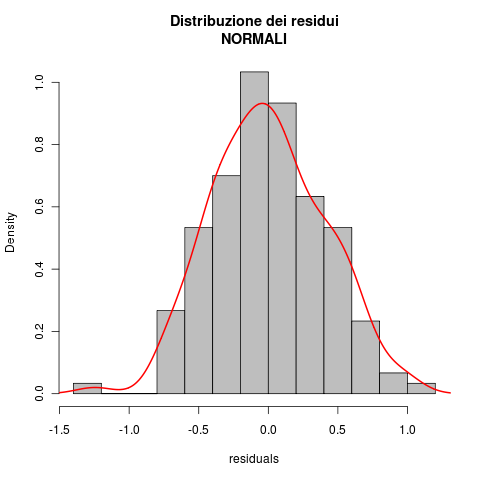
\includegraphics[height=4cm]{IstogrammaresiduiNormali.png}%
    \qquad\qquad
    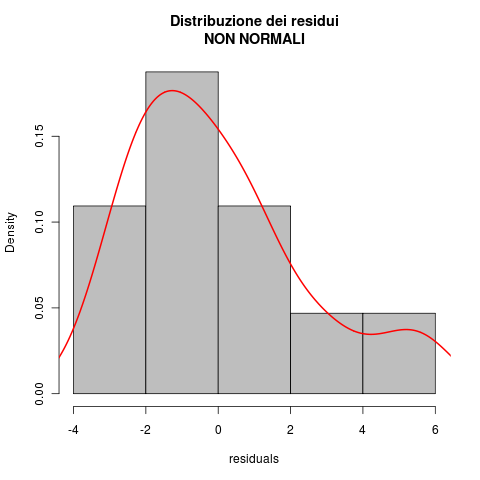
\includegraphics[height=4cm] {IstogrammaresiduiNonNormali.png}
  \end{figure}

  This kind of graphical approach is immediate, but it has to be confirmed by other tests because it is not very precise.
\end{frame}

\begin{frame}
  It can be useful to build a \textit{normal probability plot} of the residuals
  \vspace{.25cm}
  \begin{figure}[htbp]
    \centering
    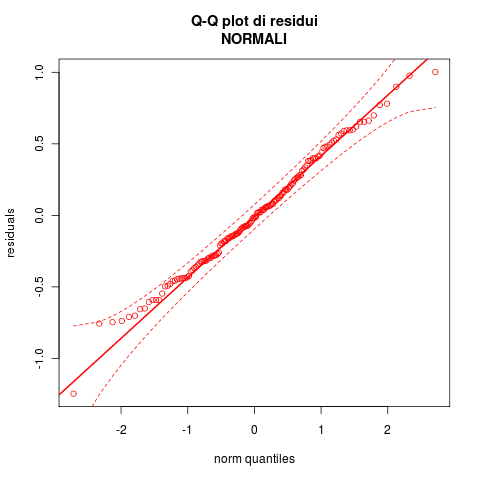
\includegraphics[scale=.30]{QQplotResiduiNormali.png}%
    \qquad\qquad
    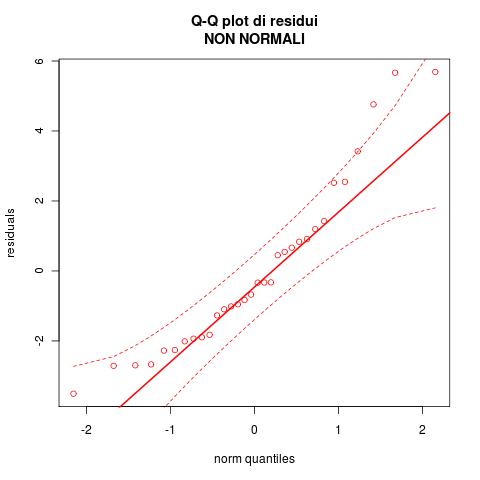
\includegraphics[scale=.30]{QQplotResiduiNonNormali.png}
  \end{figure}
  \vspace{.25cm}
  Anderson-Darling test can be used to check the normality hypothesis of the residuals.
\end{frame}

\begin{frame}
  A way to check if the formulation of the model is adequate, is that of drawing a graphic of the residuals against the estimated value of the model ($ \hat{y}_{ji} \mbox{ vs } e_{ji} $). \\
  \vspace{.25cm}
  This plot does not have to show any identifiable pattern.\\
  \vspace{.25cm}
  \begin{figure}[htbp]
    \centering
    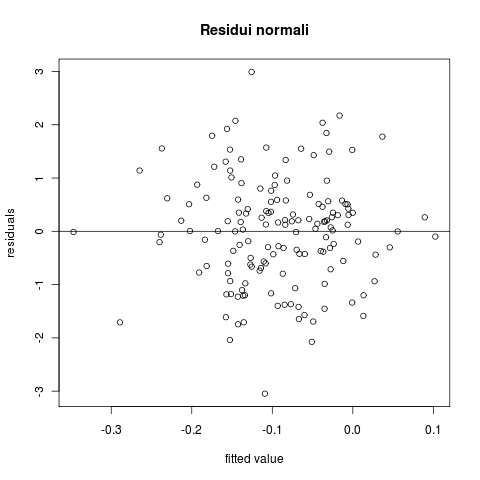
\includegraphics[height=5cm]{residuiVSFittedNormali.png}%
    \qquad\qquad
    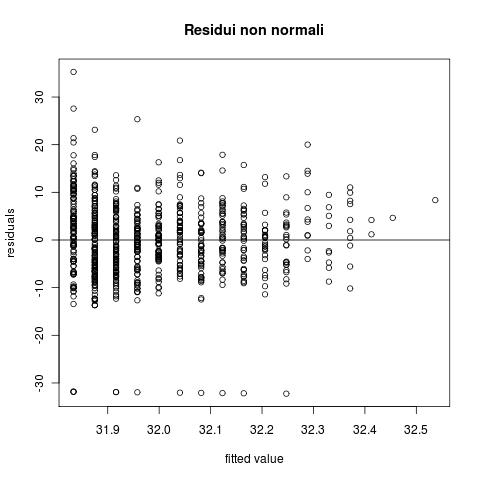
\includegraphics[height=5cm]{residuiVSFittedNonNormali.png}
  \end{figure}
\end{frame}

\begin{frame}
  Another graphic tool is the plot of the residuals against the explicative variables. The graphic does not have to show any identifiable functional trends.\\
  \vspace{0.2cm}
  If the residuals show a functional relation, it means that the linear model is not able to thoroughly explain the data.\\
  \vspace{0.75cm}
  It is useful to check that the residuals are \textbf{independent} among them. If there is autocorrelation in the residuals it means that there is dependence.
  The presence of \textbf{autocorrelation} can be caused by:
  \begin{itemize}
    \item a wrong specification of the functional link of the model;
    \item the fact that one or more explicative variables linked to the time, have not been included in the model.
  \end{itemize}
\end{frame}





\end{document}
